\documentclass[12pt,a4paper]{article}  % Use this line if this document will be released
%\documentclass[12pt,a4paper,draft]{article}  % Use this line if this document is a draft
\usepackage{ifdraft}


%% Bibliography
\usepackage{etoolbox}
\newcommand{\bibfile}{\jobname.bib}  % Name of the BibTeX file.
% ref.bib should be a symbolic link to the universal BibTeX file, which should be a local copy of
% https://github.com/equipez/bibliographie/blob/main/ref.bib
% Run `getbib` in the current directory under the draft mode to get the BibTeX file containing only
% the cited references. The name will be xyz.bib if this TeX file is xyz.tex.
\newcommand{\universalbib}{ref.bib}
\ifdraft{\IfFileExists{\universalbib}{\renewcommand{\bibfile}{\universalbib}}{}}{}
% The counter `cite' is used to count the number of citations.
\newcounter{cite}
\pretocmd{\cite}{\stepcounter{cite}}{}{}


%% Add line numbers in draft mode
\RequirePackage[mathlines]{lineno}
\ifdraft{\linenumbers}{}
\renewcommand{\linenumberfont}{\normalfont\scriptsize\sffamily\color{gray}}
\setlength{\linenumbersep}{\marginparsep}


%% Geometry
%\voffset=-1.5cm \hoffset=-1.4cm \textwidth=16cm \textheight=22.0cm  % Luis' setting
\usepackage[a4paper, textwidth=16.0cm, textheight=22.0cm]{geometry}
\renewcommand{\baselinestretch}{1.2}


%% Basic packages
\usepackage{amsmath,amsthm,amssymb,amsfonts}
\usepackage{mathtools}  % Provides \coloneqq
\usepackage{empheq}
\usepackage{xcolor}
\usepackage[bbgreekl]{mathbbol}
\DeclareSymbolFontAlphabet{\mathbbm}{bbold}
\DeclareSymbolFontAlphabet{\mathbb}{AMSb}
\usepackage{bbm}
\usepackage{upgreek}
\usepackage{accents}
\usepackage{xspace}
\usepackage{rotating}
\usepackage{multirow,booktabs}
\usepackage[en-US]{datetime2}


%% Format of the table of content
\usepackage[normalem]{ulem}
\usepackage[toc,page]{appendix}
\renewcommand{\appendixpagename}{\Large{Appendix}}
\renewcommand{\appendixname}{Appendix}
\renewcommand{\appendixtocname}{Appendix}
%\usepackage{sectsty}
\setcounter{tocdepth}{2}


%% Section title style
\usepackage{sectsty}
\sectionfont{\large}
\subsectionfont{\large}


%% Some colors
\definecolor{darkblue}{rgb}{0,0.1,0.5}
\definecolor{darkgreen}{rgb}{0,0.5,0.1}
\definecolor{darkyellow}{rgb}{0.65,0.65,0.01}


%% Todo notes
\ifdraft{
    \setlength{\marginparwidth}{2.42cm}
    \usepackage[tickmarkheight=3pt,textsize=small,backgroundcolor=blue!16,linecolor=purple,bordercolor=purple]{todonotes}
}{
    \newcommand{\todo}[1]{}
    \newcommand{\listoftodos}{}
}


%% Graph, tikz and pgf
%\usepackage{subfigure}
\setlength{\unitlength}{1mm}
% The \unitlength command is a Length command. It defines the units used in the Picture Environment.
\usepackage{graphicx}
%\usepackage{tikz,tikzscale,pgf,pgfarrows,pgfnodes,filecontents,tikz-cd}
\usepackage{tikz,tikzscale,pgf}
\usetikzlibrary{arrows,arrows.meta,patterns,positioning,decorations.markings,shapes}
\usepackage{pgfplots}
\usepackage{pgfplotstable}
\usepackage[justification=centering]{caption}
\usepgfplotslibrary{fillbetween}
\pgfplotsset{compat=1.11}

\usepackage{subcaption}
%% Turn off some unharmful warnings in draft mode
%% N.B.: DO NOT use `silence` together with `hyperref`. They will cause an infinite loop.
\ifdraft{
    \usepackage{silence}
    \WarningFilter{xcolor}{Incompatible color definition on}
    \WarningFilter{hyperref}{Draft mode on}
    \WarningFilter{refcheck}{Unused label}
    \WarningFilter{microtype}{`draft' option active}
    \WarningFilter{latex}{Writing or overwriting file} % Mute the warning about 'writing/overwriting file'
    \WarningFilter{latex}{Writing file} % Mute the warning about 'writing/overwriting file'
    \WarningFilter{latex}{Tab has} % Mute the warning about 'Tab has been converted to Blank Space'
    \WarningFilter{latex}{Marginpar on page} % Mute the warning about 'Marginpar on page xx moved'
    \WarningFilter{latex}{author given} % Mute the warning about 'No \author given'
}{}


%% Hyperref, url, and email
%% N.B.: DO NOT use `silence` together with `hyperref`. They will cause an infinite loop.
\ifdraft{\usepackage{refcheck}\newcommand{\url}{\texttt}}{
    \usepackage{hyperref}
    \hypersetup{colorlinks, linkcolor=darkblue, anchorcolor=darkblue, citecolor=darkblue, urlcolor=darkblue}
    \usepackage{url}
} % Check unused labels
\newcommand{\email}{\texttt}


%% Enumerate and itemize
\usepackage{eqlist}
\usepackage{enumitem}
\setlist[itemize]{leftmargin=*}
\setlist[enumerate]{leftmargin=*,label=\normalfont{(\alph*)}}


%% Algorithm environment
\usepackage[section]{algorithm}
\usepackage{algpseudocode,algorithmicx}
\newcommand{\INPUT}{\textbf{Input}}
\newcommand{\FOR}{\textbf{For}~}
\algrenewcommand\algorithmicrequire{\textbf{Input:}}
\algrenewcommand\algorithmicensure{\textbf{Output:}}
\algrenewcommand\alglinenumber[1]{\normalsize #1.}
\newcommand*\Let[2]{\State #1 $=$ #2}


%% Theorem-like environments
\newtheorem{theorem}{Theorem}[section]
\newtheorem{conjecture}{Conjecture}[section]
\newtheorem{corollary}{Corollary}[section]
\newtheorem{exercise}{Exercise}[section]
\newtheorem{lemma}{Lemma}[section]
\newtheorem{problem}{Problem}[section]
\newtheorem{proposition}{Proposition}[section]
\newtheorem{assumption}{Assumption}[section]
\newtheorem{example}{Example}[section]
\newtheorem{question}{Question}[section]
% Change theoremstyle to ``definition'', which uses textnormal for the text.
\theoremstyle{definition}
\newtheorem{definition}{Definition}[section]
\newtheorem{remark}{Remark}[section]
% proof
\usepackage{xpatch}
\xpatchcmd{\proof}{\itshape}{\normalfont\proofnamefont}{}{}
\newcommand{\proofnamefont}{\bfseries}

%% Equation numbering
\numberwithin{equation}{section}


%% Fine tuning
\usepackage{microtype}
\usepackage[nobottomtitles*]{titlesec} % No section title at the bottom of pages
% Prevent footnote from running to the next page
\interfootnotelinepenalty=10000
% No line break in inline math
\interdisplaylinepenalty=10000
\relpenalty=10000
\binoppenalty=10000
% No widow or orphan lines
\clubpenalty=10000
\widowpenalty=10000
\displaywidowpenalty=10000


% Use @ to put 1 math unit (mu) in math
% See https://nhigham.com/2013/01/07/fine-tuning-spacing-in-latex-equations/
% and also TeXbook p. 155.
\mathcode`@="8000{\catcode`\@=\active\gdef@{\mkern1mu}}


%% Operators, commands
\usepackage{relsize}
\usepackage{nccmath}
%\DeclareMathOperator*{\mcap}{\,\medmath{\bigcap}\,}
%\DeclareMathOperator*{\mcup}{\,\medmath{\bigcup}\,}
\DeclareMathOperator*{\mcap}{\,\mathsmaller{\bigcap}\,}
\DeclareMathOperator*{\mcup}{\,\mathsmaller{\bigcup}\,}
%\renewcommand{\cap}{\mcap}
%\renewcommand{\cup}{\mcup}

\newcommand{\ceil}[1]{ {\lceil{#1}\rceil} }
\newcommand{\floor}[1]{ {\lfloor{#1}\rfloor} }

\DeclareMathOperator{\tr}{tr}
\DeclareMathOperator{\sort}{sort}
\DeclareMathOperator*{\Argmax}{Argmax}
\DeclareMathOperator*{\Argmin}{Argmin}
\DeclareMathOperator*{\Arglocmin}{Arglocmin}
\DeclareMathOperator*{\argmax}{argmax}
\DeclareMathOperator*{\argmin}{argmin}
\DeclareMathOperator*{\diag}{diag}
\DeclareMathOperator*{\Diag}{Diag}
\DeclareMathOperator{\Span}{span}
\DeclareMathOperator{\med}{med}
\DeclareMathOperator{\essinf}{essinf}
\DeclareMathOperator{\cl}{cl}
\DeclareMathOperator{\vol}{vol}
\DeclareMathOperator{\comp}{C}
\DeclareMathOperator{\sign}{sign}
\DeclareMathOperator{\rank}{rank}
\DeclareMathOperator{\range}{range}
\DeclareMathOperator{\card}{card}
\DeclareMathOperator{\diam}{diam}
\DeclareMathOperator{\dist}{dist}
\newcommand{\disth}{{\operatorname{\updelta_{\sss{H}}}}}
\newcommand{\ind}{\mathbbm{1}}
%\newcommand*{\defeq}{\stackrel{\mbox{\normalfont\tiny{\textnormal{def}}}}{=}}
\newcommand\defeq{\mathrel{\overset{\makebox[0pt]{\mbox{\normalfont\tiny\sffamily def}}}{=}}}

\newcommand{\RR}{\mathbb{R}}
\newcommand{\BB}{\mathcal{B}}
\renewcommand{\SS}{\mathbb{S}}
\newcommand{\TT}{\mathcal{T}}
\newcommand{\ZZ}{\mathbb{Z}}
\newcommand{\NN}{\mathbb{N}}
\newcommand{\FF}{\mathcal{F}}
\newcommand{\CC}{\mathbb{C}}
\newcommand{\XX}{\mathcal{X}}
\newcommand{\sset}{\mathcal{S}}
\newcommand{\pen}{h}
\newcommand{\penpar}{\mu}
\newcommand{\res}{\rho}
\newcommand{\col}{r}
\newcommand{\ofd}{\mathcal{F}}
\newcommand{\stf}[1]{\mathbb{S}^{#1}}
\newcommand{\sss}[1]{{\scriptscriptstyle{#1}}}
\newcommand{\sK}{{\scriptscriptstyle{K}}}
\newcommand{\sT}{{\scriptscriptstyle{T}}}
\newcommand{\fro}{{\scriptstyle{\textnormal{F}}}}
\newcommand{\trs}{{\scriptstyle{\mathsf{T}}}}
\newcommand{\hmt}{{\scriptstyle{{\mathsf{H}}}}}
\newcommand{\pin}{{\scriptstyle{{\mathsf{+}}}}}
\newcommand{\inv}{{-1}}
\newcommand{\adj}{*}
\newcommand{\ones}{\mathbf{1}}

\newcommand{\cs}{\text{c}}
\newcommand{\hp}{\circ}
\newcommand{\cc}{\sss{\textnormal{C}}}
\newcommand{\dec}{\sss{\textnormal{D}}}
\newcommand{\cauchy}{\sss{\textnormal{C}}}
\newcommand{\scauchy}{\sss{\textnormal{S}}}
\newcommand{\crit}{\textnormal{crit}}
\newcommand{\rsg}{\hat{\partial}}
\newcommand{\gsg}{\partial}
\newcommand{\dom}{\textnormal{dom}}
\newcommand{\tf}{{\textnormal{f}}}
\newcommand{\tg}{{\textnormal{g}}}
\newcommand{\ts}{{\textnormal{s}}}
\newcommand{\st}{\textnormal{s.t.}}
\newcommand{\etc}{{etc.}\xspace}
\newcommand{\ie}{{i.e.}\xspace}
\newcommand{\eg}{{e.g.}\xspace}
\newcommand{\etal}{{et al.}\xspace}
\newcommand{\iid}{\text{i.i.d.}\xspace}
\newcommand{\as}{\text{a.s.}\xspace}

\newcommand{\me}{\mathrm{e}}
\newcommand{\md}{\mathrm{d}}
\newcommand{\mi}{\mathrm{i}}
\newcommand{\lev}{\mathrm{lev}}
\newcommand{\bA}{\mathbf{A}}
\newcommand{\bx}{\mathbf{u}}
%\newcommand{\bb}{\mathbf{f}}
\newcommand{\bb}{\mathbf{r}}
\newcommand{\nov}{n_{\textnormal{o}}}
\xspaceaddexceptions{]\}}
% tex.stackexchange.com/questions/15252/why-does-xspace-behave-differently-for-parenthesis-vs-braces-brackets
\newcommand{\MATLAB}{\textsc{Matlab}\xspace}
\newcommand{\octave}{\mbox{GNU Octave}\xspace}
\newcommand{\prblm}{\texttt}
\DeclareMathAlphabet{\mathsfit}{T1}{\sfdefault}{\mddefault}{\sldefault}
\SetMathAlphabet{\mathsfit}{bold}{T1}{\sfdefault}{\bfdefault}{\sldefault}
\newcommand{\prbb}{\mathsfit{p}}
\newcommand{\pp}{\mathsf{p}}
\newcommand{\qq}{\mathsf{q}}
\newcommand{\ttt}{\mathsfit{t}}
\newcommand{\tol}{\varepsilon}
\newcommand{\bt}{\mathbf{t}}
\newcommand{\br}{\mathbf{r}}
\newcommand{\dd}{\mathbf{d}}
\newcommand{\ii}{\mathbf{i}}
\newcommand{\jj}{\mathbf{j}}
\newcommand{\xx}{\mathbf{x}}
\renewcommand{\pp}{\mathbf{p}}
\renewcommand{\ggg}{\mathbf{g}}
\newcommand{\GG}{\mathbf{G}}
\DeclareMathOperator{\expc}{\mathbb{E}}
\renewcommand{\Pr}{\mathbb{P}}
\newcommand{\lb}{\underline}
\newcommand{\ub}{\overline}

% mathlcal font
\DeclareFontFamily{U}{dutchcal}{\skewchar\font=45 }
\DeclareFontShape{U}{dutchcal}{m}{n}{<-> s*[1.0] dutchcal-r}{}
\DeclareFontShape{U}{dutchcal}{b}{n}{<-> s*[1.0] dutchcal-b}{}
\DeclareMathAlphabet{\mathlcal}{U}{dutchcal}{m}{n}
\SetMathAlphabet{\mathlcal}{bold}{U}{dutchcal}{b}{n}

% mathscr font (supporting lowercase letters)
%\usepackage[scr=dutchcal]{mathalfa}
%\usepackage[scr=esstix]{mathalfa}
%\usepackage[scr=boondox]{mathalfa}
%\usepackage[scr=boondoxo]{mathalfa}
\usepackage[scr=boondoxupr]{mathalfa}
%\newcommand{\model}{\mathscr{h}}
\newcommand{\model}{\tilde{f}}
\newcommand{\rmod}{F}

\newcommand{\Set}[1]{\mathcal{#1}}
\DeclareMathAlphabet{\mathpzc}{OT1}{pzc}{m}{it} % The mathpzc font
\newcommand{\slv}{\mathpzc}
% mathpzc looks great, but it stops working on 19 Feb 2020 for no reason.
%\newcommand{\slv}{\mathscr}
\newcommand{\software}{\texttt}
\DeclareMathOperator{\eff}{\mathsf{e}\;\!}
\DeclareMathOperator{\Eff}{\mathsf{E}\;\!}
\newcommand{\out}{{\text{out}}}


%% Commands for revision
\newcommand{\red}[1]{\textcolor{red}{#1}}
\newcommand{\blue}[1]{\textcolor{blue}{#1}}
\newcommand{\green}[1]{\textcolor{darkgreen}{#1}}
\newcommand{\TYPO}[1]{{\color{orange}{#1}}}
\newcommand{\MISTAKE}[1]{{\color{violet}{#1}}}
\newcommand{\REPHRASE}[1]{{\color{darkgreen}{#1}}}
\newcommand{\REVISE}[1]{{\color{blue}{#1}}}
\newcommand{\REVISEred}[1]{{\color{red}{#1}}}
\newcommand{\COMMENT}{\todo}  % Needs the todonotes package
%\newcommand{\COMMENT}[1]{\textcolor{brown}{{\small{(comment: #1)}}}}  % This puts comments inline

% Use the following if revision is finished
%\newcommand{\TYPO}{}
%\newcommand{\MISTAKE}{}
%\newcommand{\REPHRASE}{}
%\newcommand{\REVISE}{}
%\newcommand{\REVISEred}{}
%\newcommand{\COMMENT}[1]{}  % Input ignored.


%%%%%%%%%%%%%%%%%%%%%%%%%%%%%%%%%%%%%%%%%%%%%%%%%%%%%%%%%%%%%%%%%%%%%%%%%%%%%%%%%%%%%%%%%%%%%%%%%%%%
\title{Tests of PRIMA and OptiProfiler}

\date{\DTMnow}

\author{
    Zhuhuatao
    %\thanks{}
    %\and
    %Author2
    %\thanks{Information2}
}


\begin{document}

\maketitle

%\begin{abstract}
%\end{abstract}

%\textbf{Keywords}: Keyword1, Keyword2
%%%%%%%%%%%%%%%%%%%%%%%%%%%%%%%%%%%%%%%%%%%%%%%%%%%%%%%%%%%%%%%%%%%%%%%%%%%%%%%%%%%%%%%%%%%%%%%%%%%%

This is a summary of tests of PRIMA and OptiProfiler. We conduct the tests in MATLAB~R2026a.

\section{Preparation}

\subsection{PRIMA}

PRIMA is a package for solving general nonlinear optimization problems without using derivatives. It provides the reference implementation for Powell's renowned derivative-free optimization methods including COBYLA, NEWUOA, BOBYQA, and LINCOA. The ``P'' in the name stands for Powell, and ``RIMA'' is an acronym for ``\textbf{R}eference \textbf{I}mplementation with \textbf{M}odification and \textbf{A}melioration''.\footnote{See~\url{https://github.com/libprima/prima}}

To use PRIMA in MATLAB, we first download the package from GitHub by running
\begin{verbatim}
git clone https://github.com/libprima/prima.git
\end{verbatim}
in Bash. Then, after changing the current directory to~\path{path/to/prima/matlab} in MATLAB, run 
\begin{verbatim}
options.debug=true; options.single=true; options.quadruple=true; 

setup(options); testprima
\end{verbatim}
to install PRIMA and verify the installation by running the test suite.
%\newpage
We can get help by running 
\begin{verbatim}
help prima
\end{verbatim}
in MATLAB. 

\subsection{OptiProfiler}

OptiProfiler is a platform for benchmarking optimization solvers in the cloud.\footnote{See \url{https://www.optprof.com/}} For a detailed introduction, see~\cite{key}.
To use OptiProfiler in MATLAB, we first clone the repository using the following command
\begin{verbatim}
git clone https://github.com/optiprofiler/optiprofiler.git
\end{verbatim}
Then, in MATLAB, after navigating to the folder where the source code is located, run the following command in the MATLAB command window:
\begin{verbatim}
setup
\end{verbatim}
to add the source code to the MATLAB path. 




\section{Tests of PRIMA}

We use the Rosenbrock function\footnote{See \url{https://docs.scipy.org/doc/scipy-0.14.0/reference/tutorial/optimize.html\#unconstrained-minimization-of-multivariate-scalar-functions-minimize}} as the test function. The function is defined as 
\begin{equation}
    f(x) = \sum_{i=1}^{n-1} \left[ 100(x_{i+1} - x_i^2)^2 + (1 - x_i)^2 \right],
\end{equation}
where~$n$ is the dimension of the function and~$x = (x_1, x_2, \ldots, x_n)^T$. The function has a global minimum at~$x^* = (1, 1, \ldots, 1)^T$ with~$f(x^*) = 0$. We choose the dimension of the function as~$n = 50$ and the initial point as~$x_0 = (-1, -1, \ldots, -1)^T$. We apply PRIMA to the Rosenbrock function in the following cases:
\begin{itemize}
    \item Case 1: no constraints.
    \item Case 2: bound constraints:~$x \leq 0$.
    \item Case 3: linear constraints:~$\sum_{i=1}^n  x_i \leq 1$ and~$x \geq 0$.
    \item Case 4: nonlinear constraints:~$\sum_{i=1}^n  x_i^2 \leq 1$ and~$x \geq 0$.
\end{itemize}
We summarize the main results in Table~\ref{tab:prima_rosenbrock_results}. The complete results are available in the file~\path{/path/to/prima/prima_rosenbrock_results/prima_rosenbrock_results.mat}. 

In the unconstrained case, PRIMA reaches the global minimum with a very small function value. In other cases, the optimal point is out of the feasible region. PRIMA reaches the optimal values under the given constraints, which are much larger than the global minimum. In addition, since the feasible region of the nonlinear-constraint case is smaller than that of the linear-constraint case, the optimal value under the nonlinear-constraint case is larger than that under the linear-constraint case.

\begin{table}[t]
    \centering
    \caption{Results of PRIMA on the Rosenbrock function.}
    \label{tab:prima_rosenbrock_results}
    \begin{tabular}{ccccc}
        \toprule
        \textbf{Case} & \textbf{Iterations} & \textbf{Function Evaluations} & \textbf{Final Value} & \textbf{Exit Flag} \\
        \midrule
        No constraints & 3138& 3138 &  4.9602e-10 & 0  \\
        $x \leq 0$ & 779 & 779 &  49 & 0 \\
        $\sum_{i=1}^n x_i \leq 1, x \geq 0$ & 647 & 647 &  47.0965 & 0 \\
        $\sum_{i=1}^n x_i^2 \leq 1, x \geq 0$ & 1650 & 1650 &  38.8192 & 0 \\
        \bottomrule
    \end{tabular}
\end{table}

\section{Tests of OptiProfiler}

We conduct two groups of tests to compare PRIMA using the S2MPJ problem library, with a total of 515 problems selected. 
In both tests, the problem type is set to~\texttt{ubln}, which means that unconstrained, bound-constrained, linearly constrained, and nonlinearly constrained problems are tested together. 
The dimensions of the test problems range from~2 to~20. 
For each test, we consider two problem features, namely~\texttt{plain} and~\texttt{noisy}. Under the noisy feature, we run each problem three times per case. Overall, PRIMA performs better in the plain feature than in the noisy feature.

\subsection{Double and single precision}

In the first test, we compare PRIMA in double precision with PRIMA in single precision. 
The first solver is PRIMA with the option~\texttt{precision} set to~\texttt{'double'}, while the second solver is PRIMA with~\texttt{precision} set to~\texttt{'single'}.
\begin{table}[htbp]
    
    \centering
    \caption{Scores for double and single precision.}
    \label{tab:diff_precision_results}
    
    \begin{tabular}{ccc}
        \toprule
        \textbf{Feature} & \textbf{Double precision} & \textbf{Single precision}   \\
        \midrule
        plain & 1.0000& 0.8375  \\
        noisy & 1.0000& 0.9400  \\
        \bottomrule
    \end{tabular}
    
\end{table}
The relative scores are shown in Table~\ref{tab:diff_precision_results}. PRIMA achieves a higher score in double precision, especially under the plain feature.
Figure~\ref{fig:test1} shows the data profiles, log-ratio profiles, and performance profiles for the two solvers under the two features.
The blue line represents PRIMA in double precision, and the red line represents PRIMA in single precision. 
From Figures~\ref{fig:data_plain} and~\ref{fig:data_noisy}, we can see that PRIMA can solve a larger number of problems in double precision compared to single precision with the same budget of simplex gradients. In terms of the number of problems solved, PRIMA performs better in double precision than in single precision. It is more noticeable in the plain feature than in the noisy feature. When we focus on log-ratio profiles in Figures~\ref{fig:log-ratio_plain} and~\ref{fig:log-ratio_noisy}, the situation is a little different. PRIMA in double precision can solve more problems than PRIMA in single precision, especially under the plain feature. However, for the problems that can be solved by both solvers in the noisy feature, PRIMA in single precision requires fewer evaluations than PRIMA in double precision on more problems. Under the plain feature, the two solvers are evenly matched.

\begin{figure}[htbp]
    \centering

    \begin{subfigure}[t]{0.48\textwidth}
        \centering
        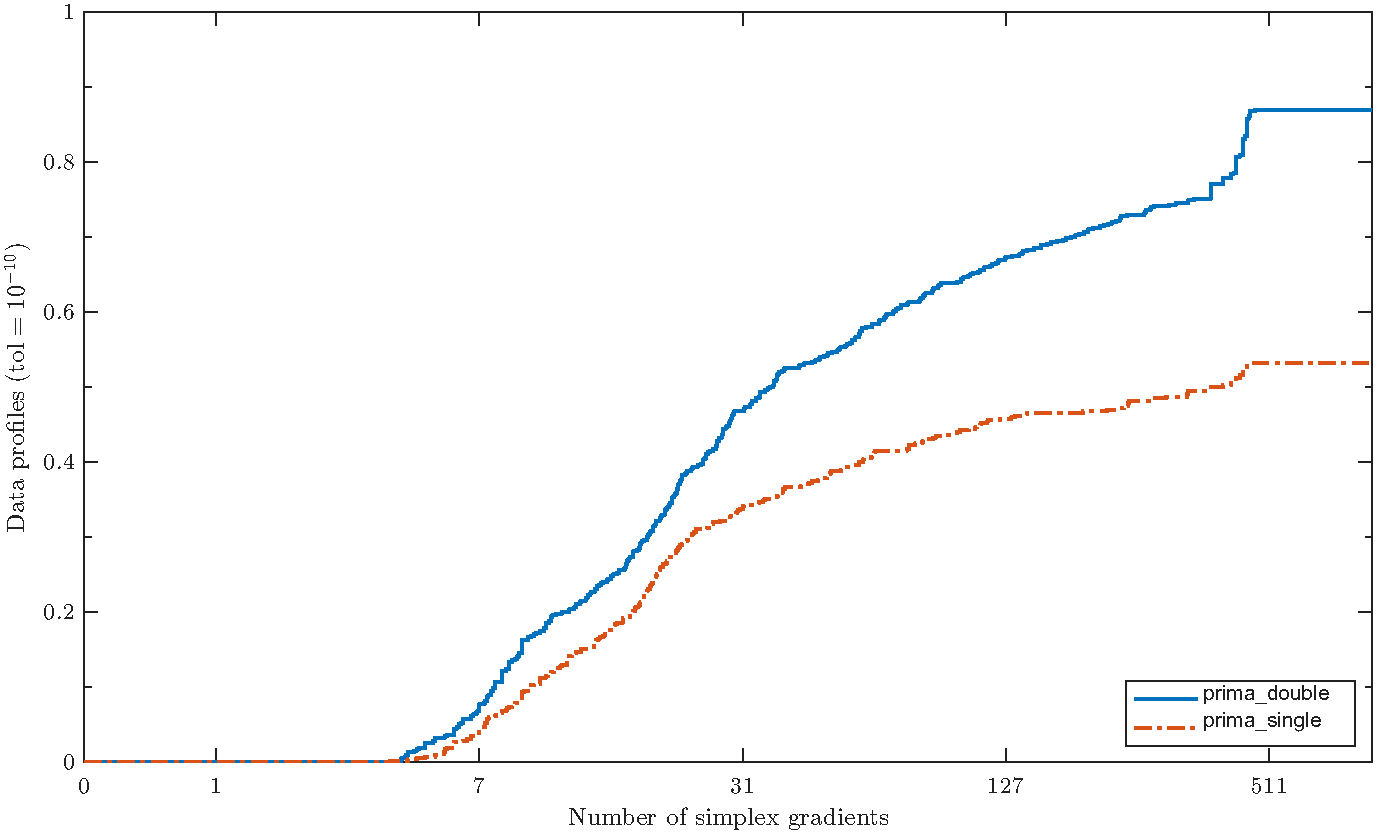
\includegraphics[width=\linewidth]{./results/optiprofiler_prima/prima_double_prima_single_ubln_2_20_0_10_plain/detailed_profiles/data_output-based/data_out_10.pdf}
        \caption{Output-based data profile for the plain feature.}
        \label{fig:data_plain}
    \end{subfigure}
    \hfill
    \begin{subfigure}[t]{0.48\textwidth}
        \centering
        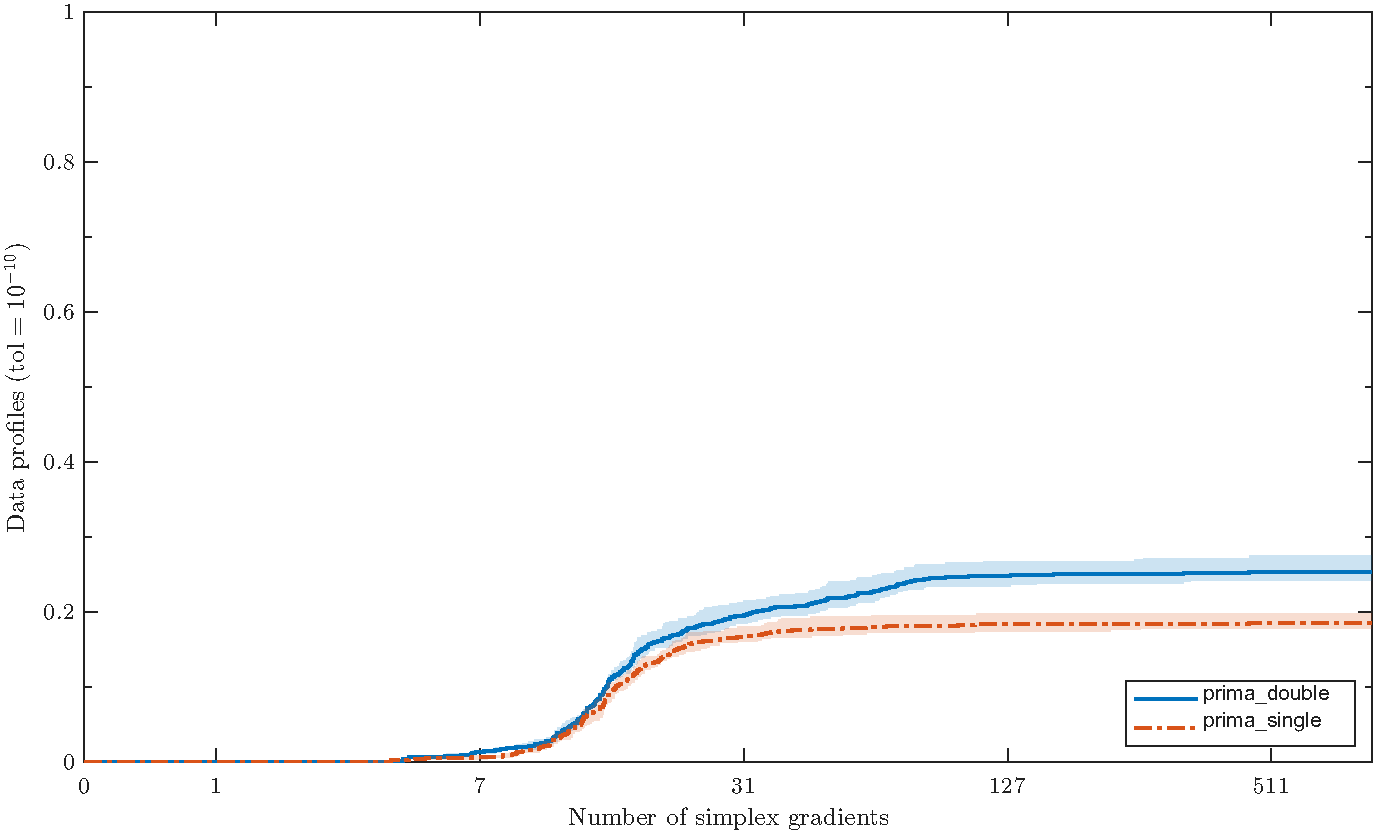
\includegraphics[width=\linewidth]{./results/optiprofiler_prima/prima_double_prima_single_ubln_2_20_0_10_noisy/detailed_profiles/data_output-based/data_out_10.pdf}
        \caption{Output-based data profile for the noisy feature.}
        \label{fig:data_noisy}
    \end{subfigure}

    \vspace{0.5em}

    \begin{subfigure}[t]{0.48\textwidth}
        \centering
        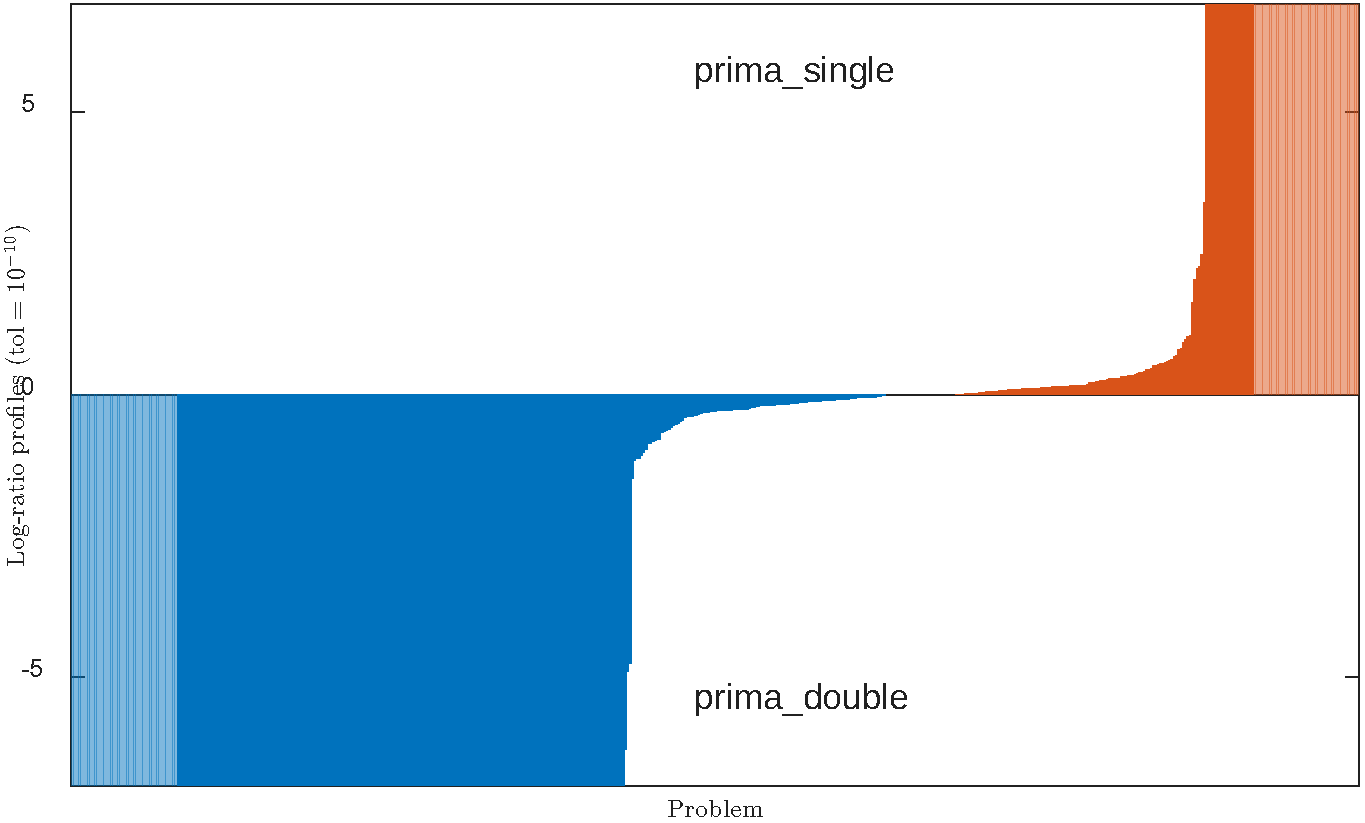
\includegraphics[width=\linewidth]{./results/optiprofiler_prima/prima_double_prima_single_ubln_2_20_0_10_plain/detailed_profiles/log-ratio_output-based/log-ratio_out_10.pdf}
        \caption{Output-based log-ratio profile for the plain feature.}
        \label{fig:log-ratio_plain}
    \end{subfigure}
    \hfill
    \begin{subfigure}[t]{0.48\textwidth}
        \centering
        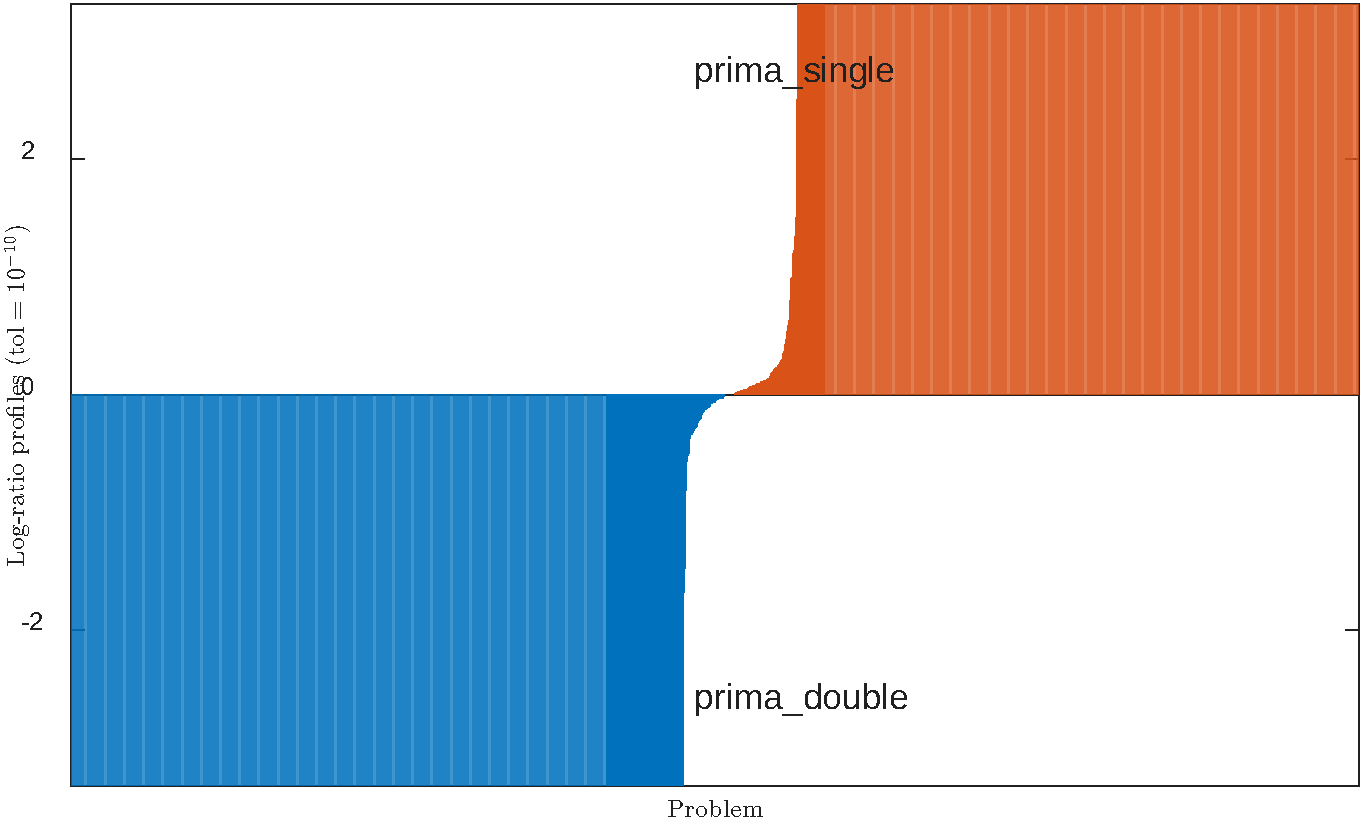
\includegraphics[width=\linewidth]{./results/optiprofiler_prima/prima_double_prima_single_ubln_2_20_0_10_noisy/detailed_profiles/log-ratio_output-based/log-ratio_out_10.pdf}
        \caption{Output-based log-ratio profile for the noisy feature.}
        \label{fig:log-ratio_noisy}
    \end{subfigure}

    \vspace{0.5em}

    \begin{subfigure}[t]{0.48\textwidth}
        \centering
        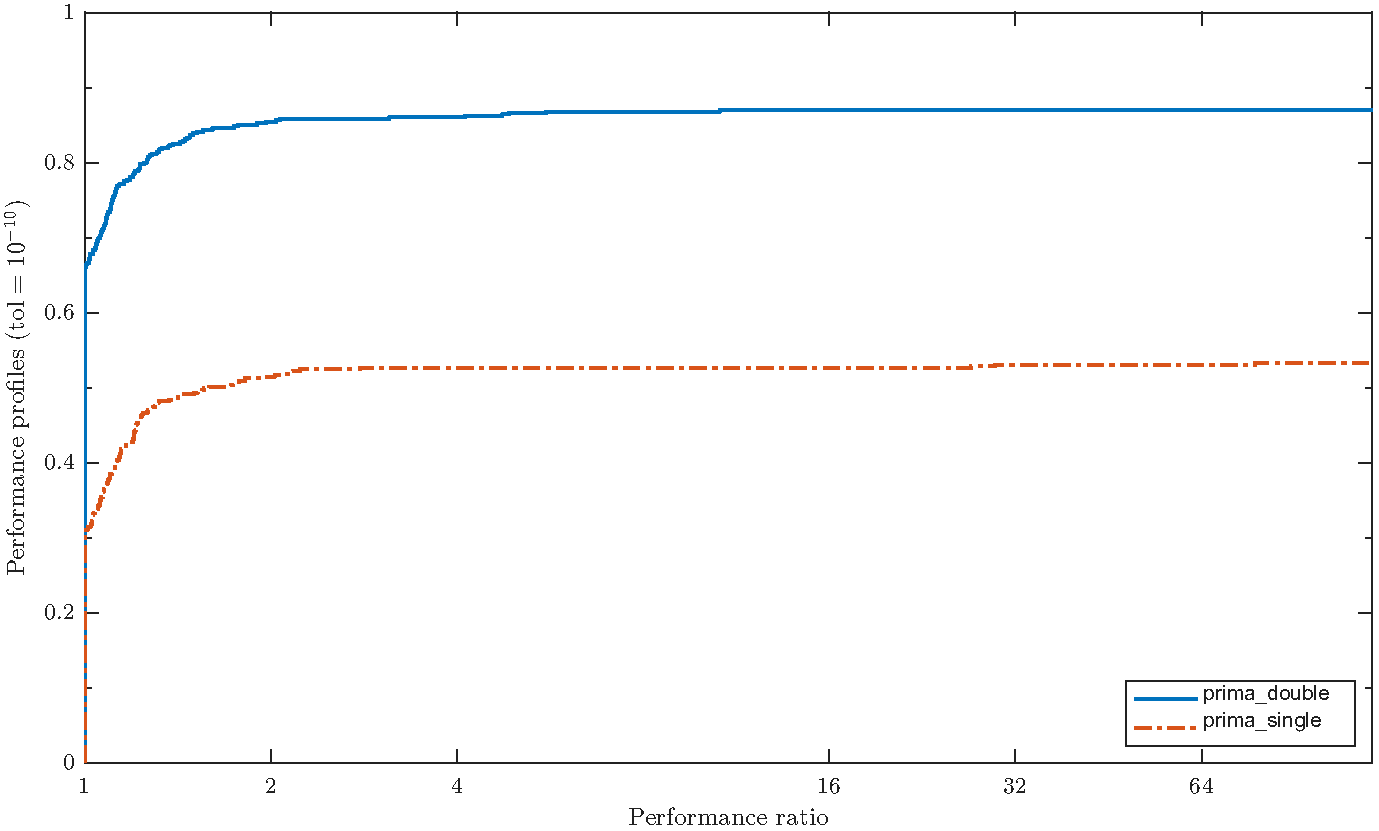
\includegraphics[width=\linewidth]{./results/optiprofiler_prima/prima_double_prima_single_ubln_2_20_0_10_plain/detailed_profiles/perf_output-based/perf_out_10.pdf}
        \caption{Output-based performance profile for the plain feature.}
        \label{fig:perf_plain}
    \end{subfigure}
    \hfill
    \begin{subfigure}[t]{0.48\textwidth}
        \centering
        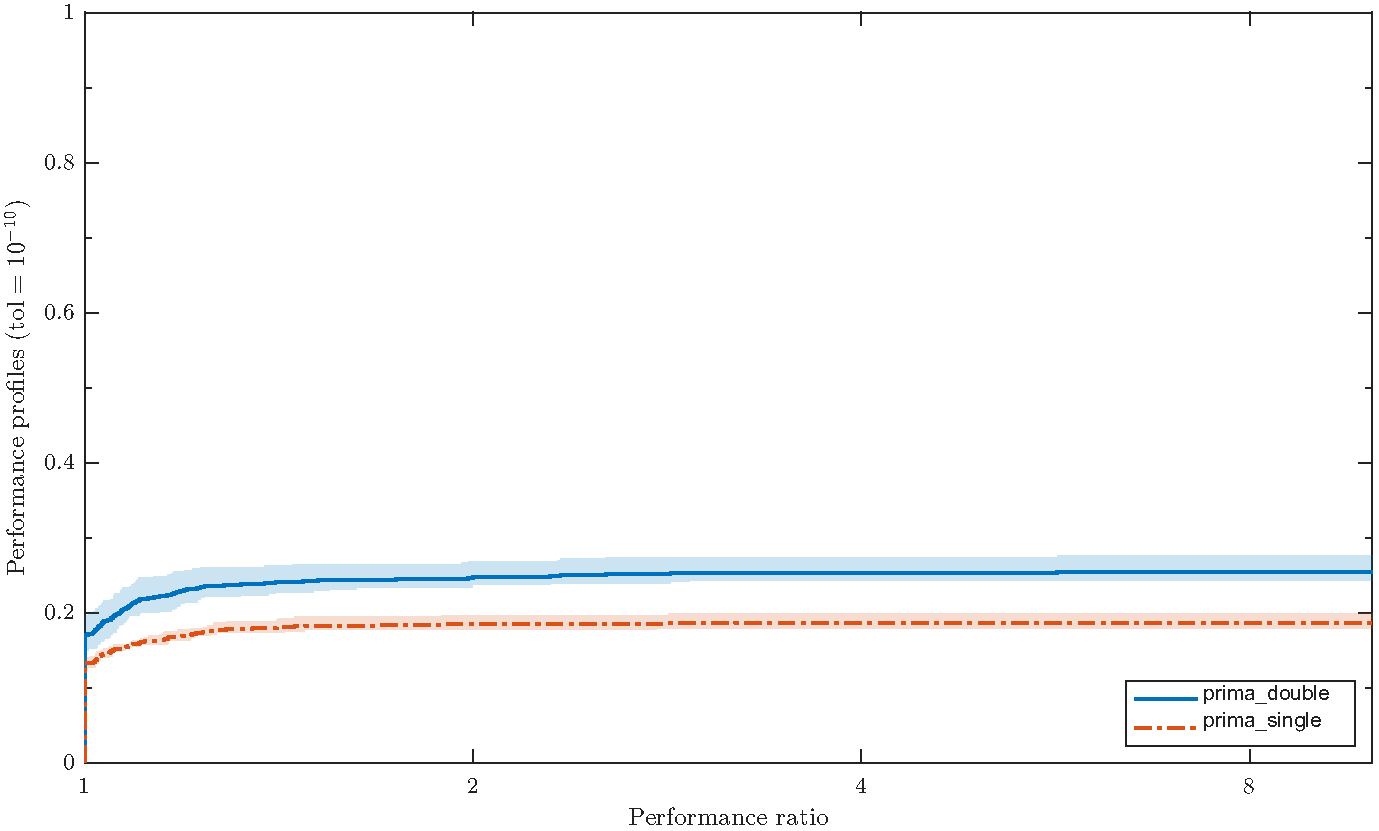
\includegraphics[width=\linewidth]{./results/optiprofiler_prima/prima_double_prima_single_ubln_2_20_0_10_noisy/detailed_profiles/perf_output-based/perf_out_10.pdf}
        \caption{Output-based performance profile for the noisy feature.}
        \label{fig:perf_noisy}
    \end{subfigure}

    \caption{Output-based data, log-ratio, and performance profiles for PRIMA in double and single precision under the \texttt{plain} and \texttt{noisy} features with~$\tau = 10^{-10}$.}
    \label{fig:test1}
\end{figure}

%\newpage

\subsection{Double and quadruple precision}

In the second test, we compare PRIMA in double precision with PRIMA in quadruple precision. 
The first solver is again PRIMA with~\texttt{precision} set to~\texttt{'double'}, while the second solver is PRIMA with~\texttt{precision} set to~\texttt{'quadruple'}.

The results are similar to those in the first test. In the plain case, PRIMA achieves higher scores as the arithmetic precision increases. In the noisy case, PRIMA with quadruple precision shows a slightly lower score than PRIMA with double precision, as shown in Figure~\ref{fig:test2}. Figure~\ref{fig:test2} shows the data profiles, log-ratio profiles, and performance profiles for the two solvers under the two features. The blue line represents PRIMA in double precision, and the red line represents PRIMA in quadruple precision. 
The similarity can also be observed in the log-ratio profiles in Figures~\ref{fig1:log-ratio_plain} and~\ref{fig1:log-ratio_noisy}. PRIMA in quadruple precision can solve more problems than PRIMA in double precision. Under the plain feature, for the problems that can be solved by both solvers, the two solvers solve a similar number of problems with fewer evaluations than the other solver. Under the noisy feature, PRIMA in quadruple precision has more problems that can be solved with fewer evaluations than PRIMA in double precision.
\begin{table}[htbp]
    
    \centering
    \caption{Scores for double and quadruple precision.}
    \label{tab:quad_precision_results}
    
    \begin{tabular}{ccc}
        \toprule
        \textbf{Feature} & \textbf{Double precision} & \textbf{Quadruple precision}   \\
        \midrule
        plain & 0.9914& 1.0000  \\
        noisy & 1.0000& 0.9692  \\
        \bottomrule
    \end{tabular}
    
\end{table}

\begin{figure}[htbp]
    \centering

    \begin{subfigure}[t]{0.48\textwidth}
        \centering
        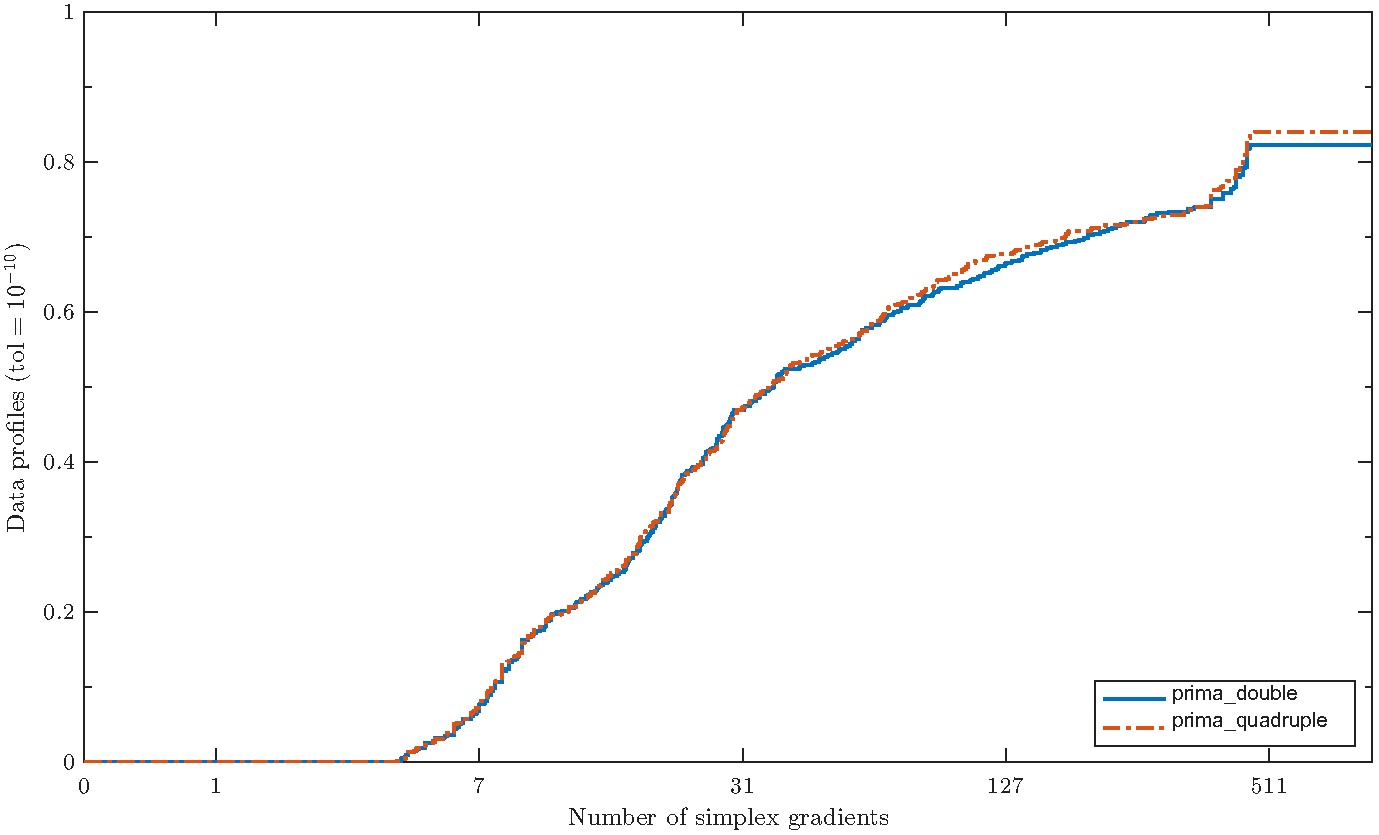
\includegraphics[width=\linewidth]{./results/optiprofiler_prima/prima_double_prima_quadruple_ubln_2_20_0_10_plain/detailed_profiles/data_output-based/data_out_10.pdf}
        \caption{Output-based data profile for the plain feature.}
        \label{fig1:data_plain}
    \end{subfigure}
    \hfill
    \begin{subfigure}[t]{0.48\textwidth}
        \centering
        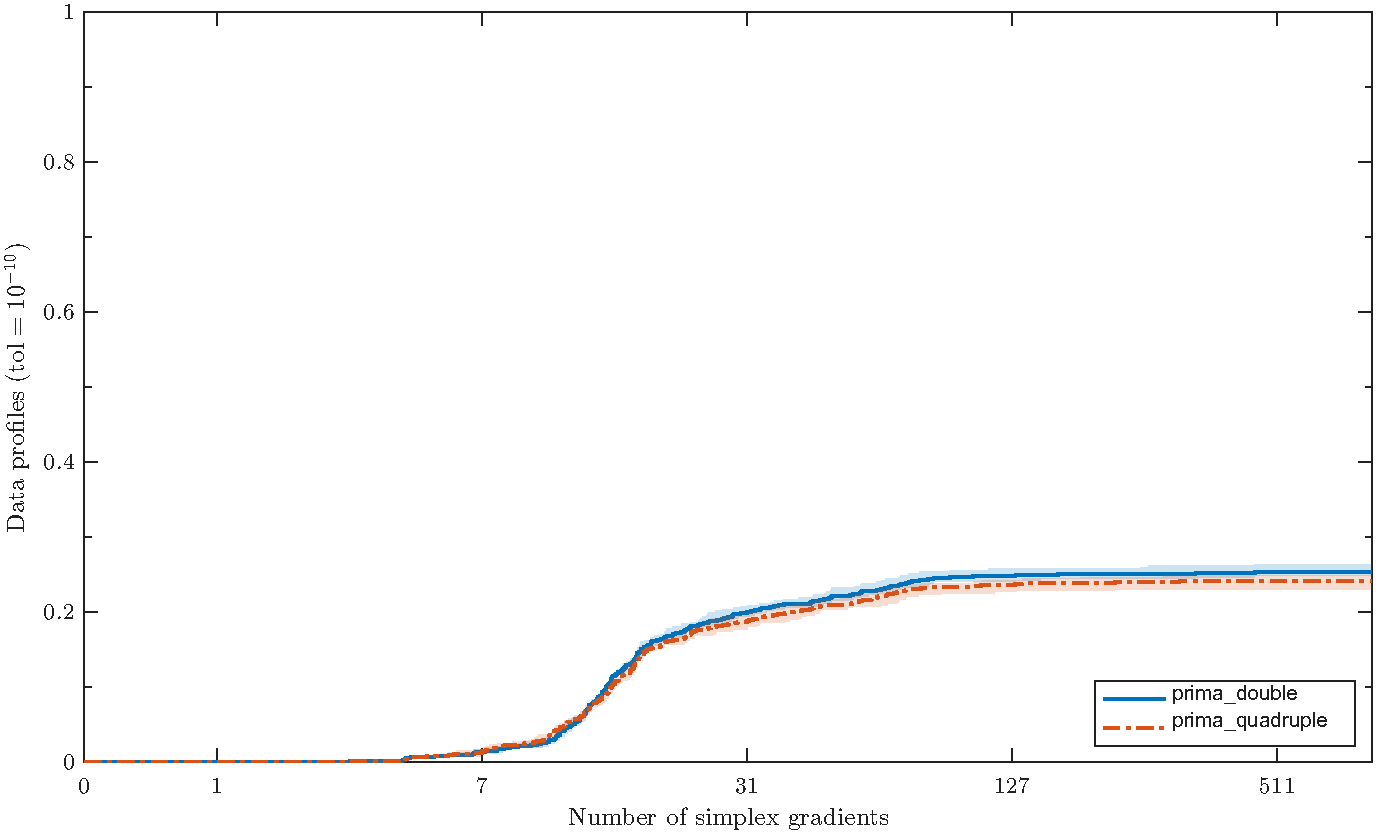
\includegraphics[width=\linewidth]{./results/optiprofiler_prima/prima_double_prima_quadruple_ubln_2_20_0_10_noisy/detailed_profiles/data_output-based/data_out_10.pdf}
        \caption{Output-based data profile for the noisy feature.}
        \label{fig1:data_noisy}
    \end{subfigure}

    \vspace{0.5em}

    \begin{subfigure}[t]{0.48\textwidth}
        \centering
        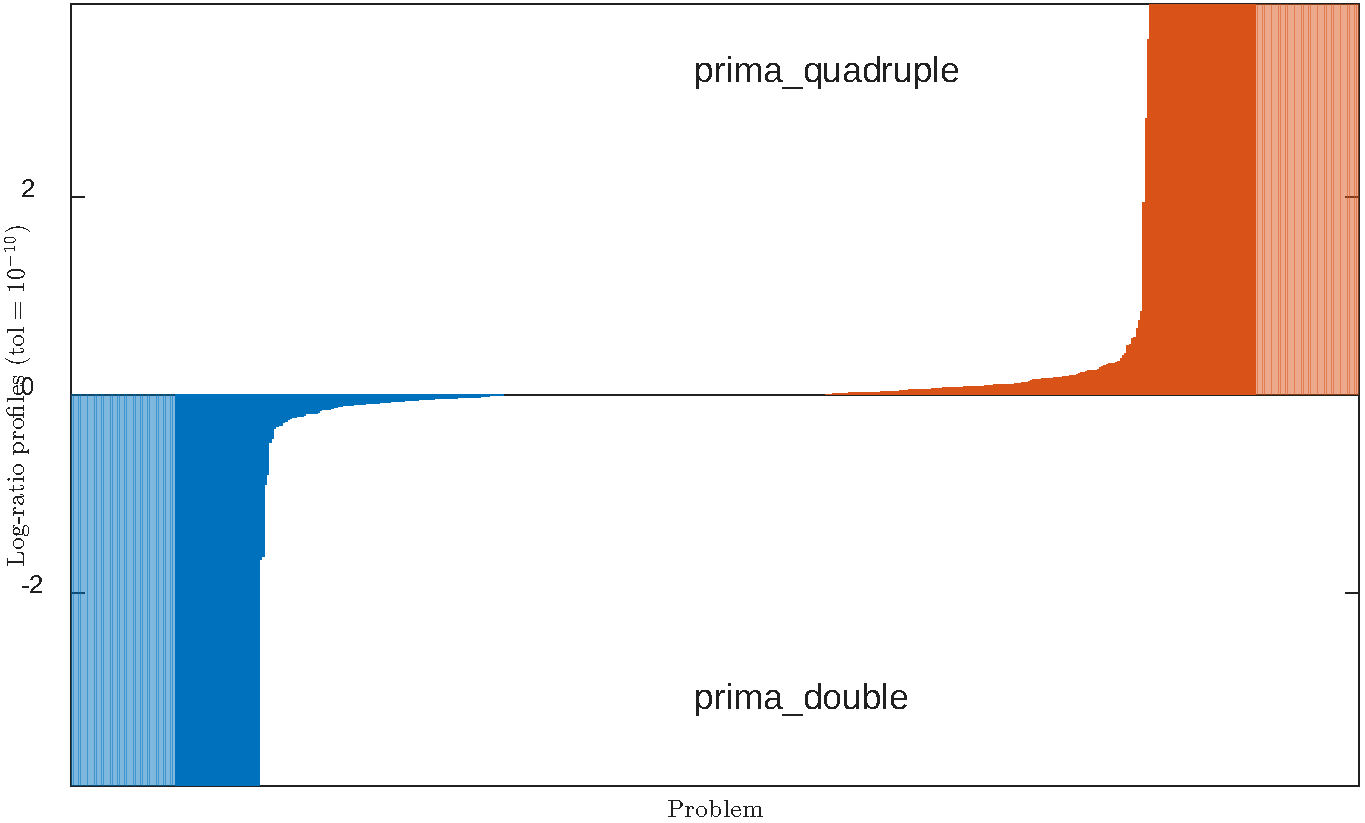
\includegraphics[width=\linewidth]{./results/optiprofiler_prima/prima_double_prima_quadruple_ubln_2_20_0_10_plain/detailed_profiles/log-ratio_output-based/log-ratio_out_10.pdf}
        \caption{Output-based log-ratio profile for the plain feature.}
        \label{fig1:log-ratio_plain}
    \end{subfigure}
    \hfill
    \begin{subfigure}[t]{0.48\textwidth}
        \centering
        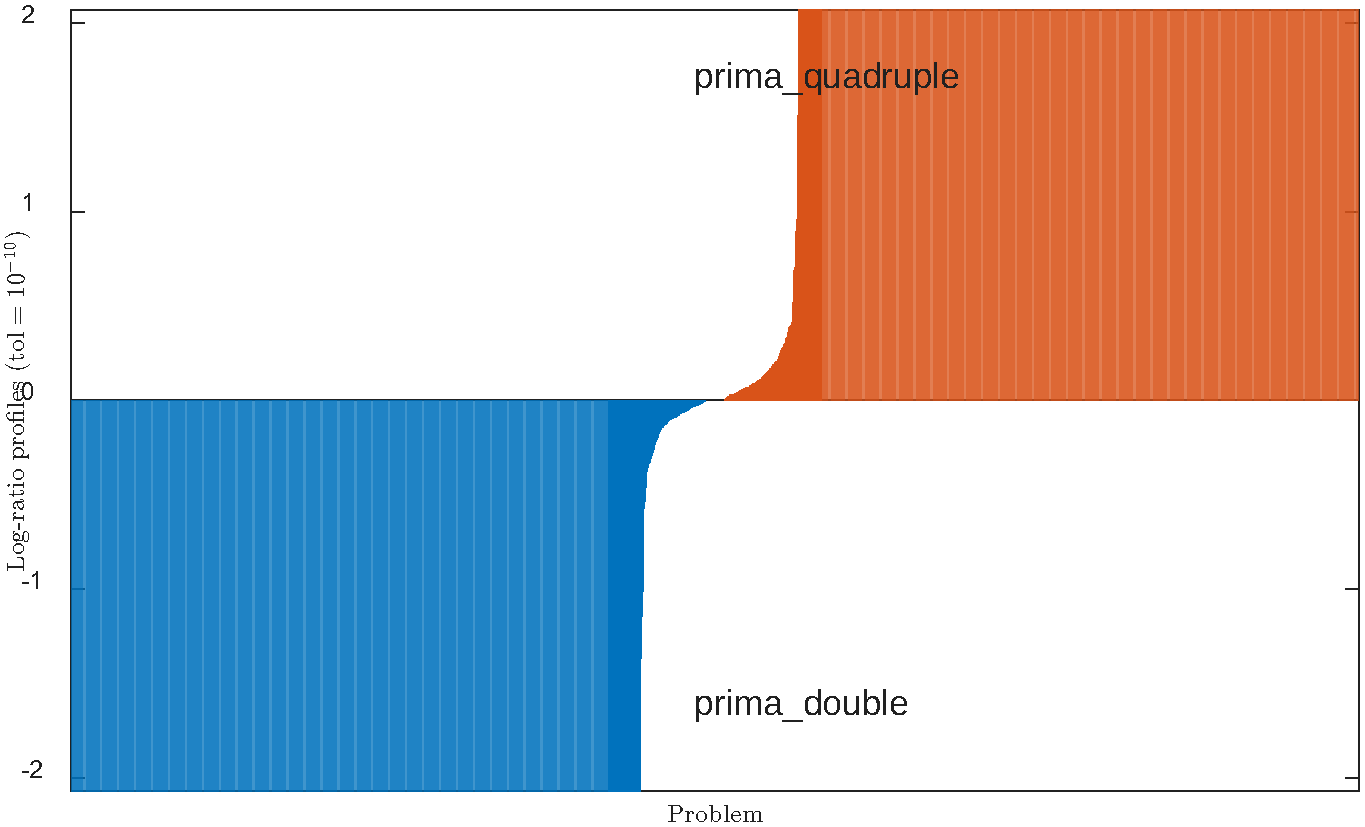
\includegraphics[width=\linewidth]{./results/optiprofiler_prima/prima_double_prima_quadruple_ubln_2_20_0_10_noisy/detailed_profiles/log-ratio_output-based/log-ratio_out_10.pdf}
        \caption{Output-based log-ratio profile for the noisy feature.}
        \label{fig1:log-ratio_noisy}
    \end{subfigure}

    \vspace{0.5em}

    \begin{subfigure}[t]{0.48\textwidth}
        \centering
        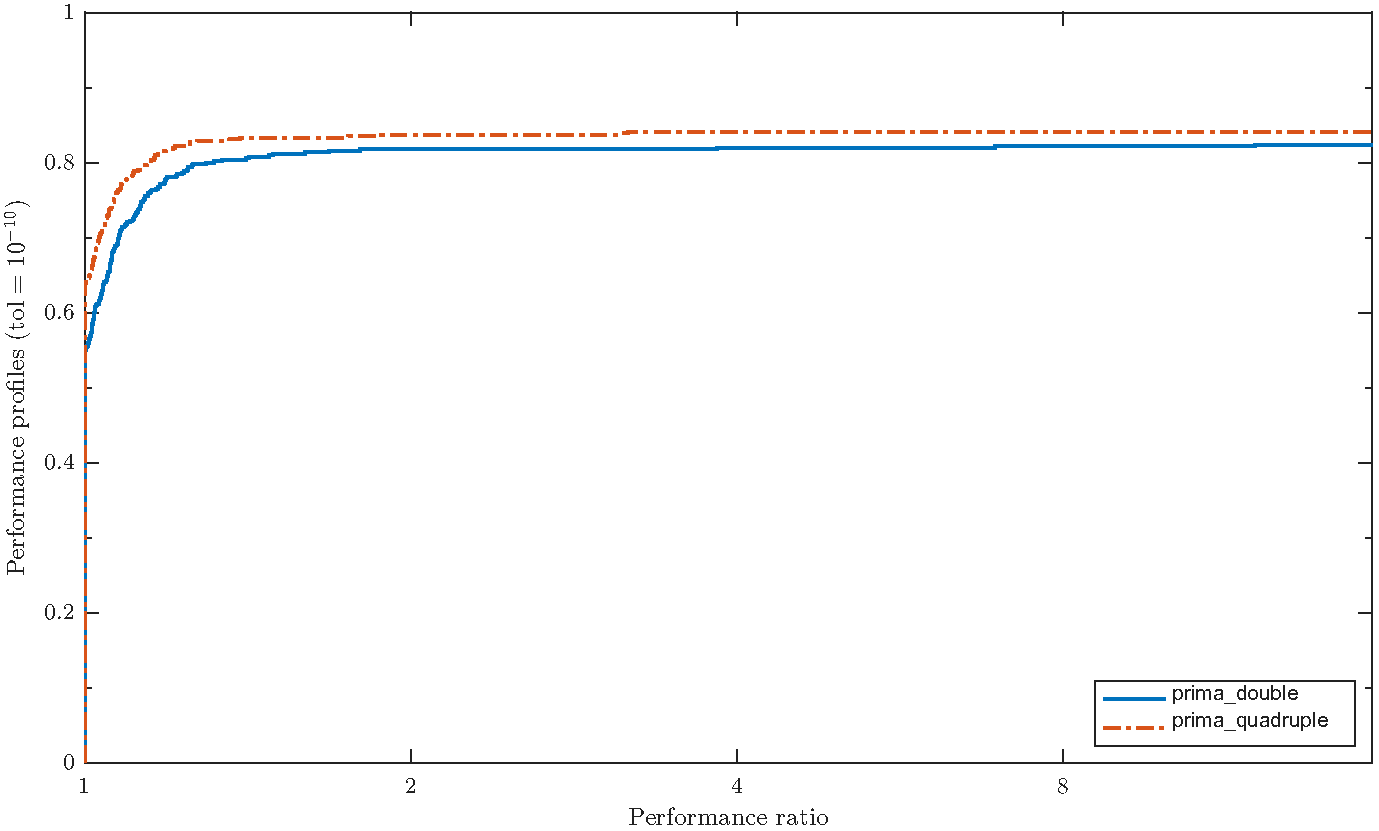
\includegraphics[width=\linewidth]{./results/optiprofiler_prima/prima_double_prima_quadruple_ubln_2_20_0_10_plain/detailed_profiles/perf_output-based/perf_out_10.pdf}
        \caption{Output-based performance profile for the plain feature.}
        \label{fig1:perf_plain}
    \end{subfigure}
    \hfill
    \begin{subfigure}[t]{0.48\textwidth}
        \centering
        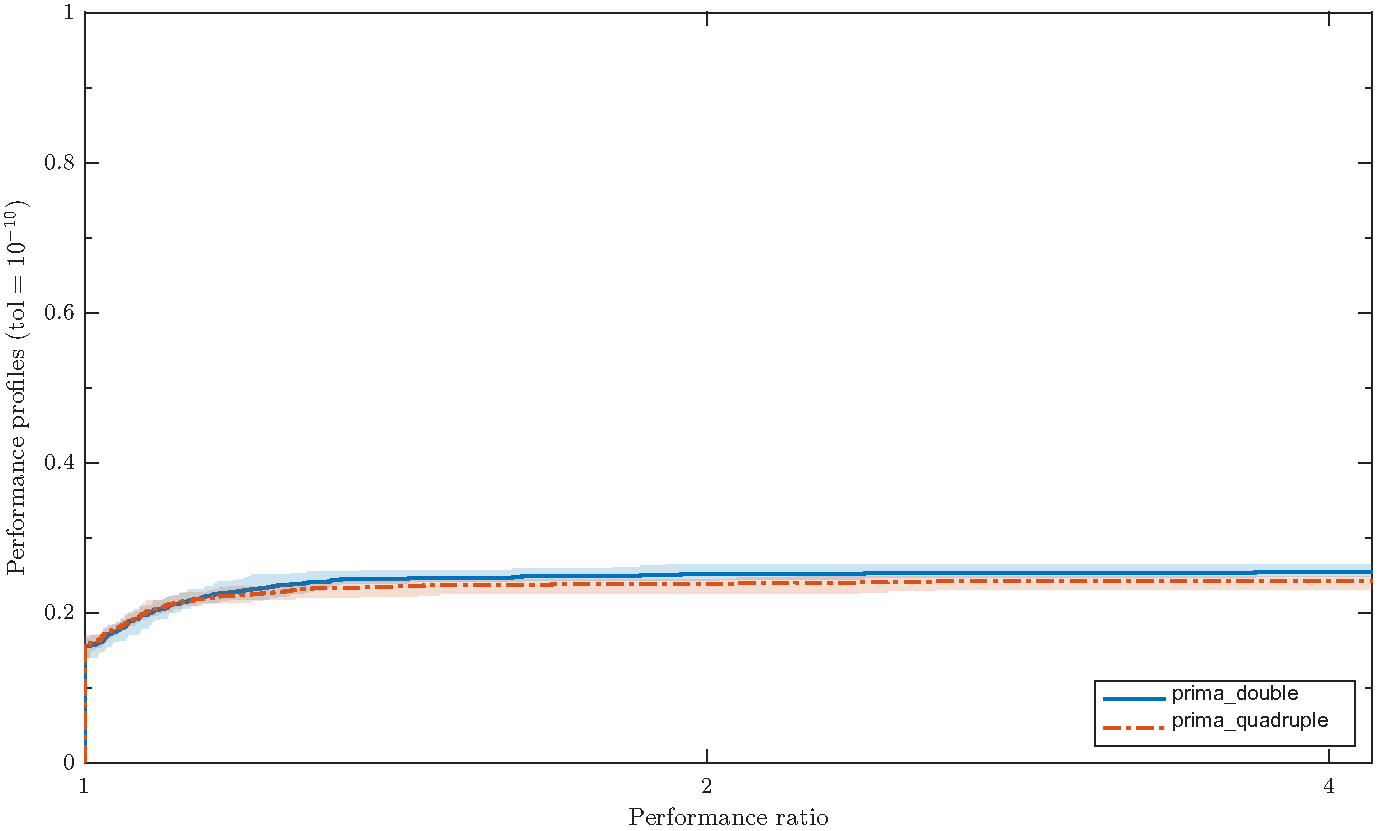
\includegraphics[width=\linewidth]{./results/optiprofiler_prima/prima_double_prima_quadruple_ubln_2_20_0_10_noisy/detailed_profiles/perf_output-based/perf_out_10.pdf}
        \caption{Output-based performance profile for the noisy feature.}
        \label{fig1:perf_noisy}
    \end{subfigure}

    \caption{Output-based data, log-ratio, and performance profiles for PRIMA in double and quadruple precision under the \texttt{plain} and \texttt{noisy} features with~$\tau = 10^{-10}$.}
    \label{fig:test2}
\end{figure}

\subsection{Conclusion}

When comparing different arithmetic precisions, PRIMA achieves higher scores in higher precision, especially under the plain feature. In the noisy feature, PRIMA with lower precision performs better in relative scores. In the comparison sense represented by Figures~\ref{fig:test1} and~\ref{fig:test2}, PRIMA with double precision has better performance than PRIMA with single precision, while the advantage of PRIMA with quadruple precision over PRIMA with double precision is not significant.
The improvement of PRIMA with higher precision is significant in the plain feature but is not obvious in the noisy feature. The noise has a larger impact on the performance of PRIMA than the arithmetic precision.



%%%%%%%%%%%%%%%%%%%%%%%%%%%%%%%%%%%%%%%%%%%%%%%%%%%%%%%%%%%%%%%%%%%%%%%%%%%%%%%%%%%%%%%%%%%%%%%%%%%%
%% References
% Include references only if there are citations.
\ifnum\value{cite}>0
    \small
    \bibliography{reference}
    \bibliographystyle{plain}
\fi

%% The end
\end{document}
